\documentclass[runningheads]{llncs}

\usepackage{graphicx}
\usepackage{amsmath}
\usepackage{amssymb}
\usepackage{booktabs}
\usepackage{array}
\usepackage{url}
\usepackage{placeins}
\setlength{\textfloatsep}{8pt plus 1pt minus 2pt}
\setlength{\floatsep}{7pt plus 1pt minus 2pt}
\setlength{\intextsep}{7pt plus 1pt minus 2pt}
\setlength{\abovecaptionskip}{4pt}
\setlength{\belowcaptionskip}{0pt}

\newcommand{\figplaceholder}[2]{%
\fbox{%
\begin{minipage}[c][0.20\textheight][c]{0.92\textwidth}
\centering
\textbf{#1}\\[0.8em]
#2
\end{minipage}}}

\begin{document}

\title{Region-Temporal Attention Multi-Region Color Pulse Network for Contactless Stress Recognition}
\titlerunning{RT-MRCPNet for Contactless Stress Recognition}

\author{Anonymous Authors}
\authorrunning{Anonymous Authors}
\institute{Anonymous Institution}

\maketitle

\begin{abstract}
Stress often appears physiologically before it is obvious in facial expression or behavior. Facial-video stress recognition is contactless and unobtrusive, but useful skin-color changes are weak, spatially uneven, and easily masked by motion, illumination, and subject appearance. Full-frame facial modeling may learn identity or scene shortcuts on small datasets, whereas recovering one whole-face physiological signal can discard regional differences too early. To address these issues, this paper proposes RT-MRCPNet, a Region-Temporal Attention Multi-Region Color Pulse Network. It converts each facial clip into multi-region color sequences and treats the regions as weak physiological observations. A shared temporal encoder extracts regional color dynamics, temporal attention selects reliable segments within each region, and region attention fuses facial areas into a clip-level stress representation. Under a subject-independent protocol on social-stress facial video data, RT-MRCPNet achieves 86.42\% accuracy, 90.27\% F1-score, and 93.07\% area under the curve; compared with fixed multi-region fusion, it improves the three metrics by 5.70, 4.60, and 3.95 percentage points. The results show that adaptive temporal and regional weighting outperforms full-face color sequences, single-region sequences, hand-crafted remote photoplethysmography features, and lightweight neural baselines.

\keywords{Contactless stress \and Regional color sequences \and Region-temporal attention \and Physiological visual representation \and Cross-subject evaluation}
\end{abstract}

\section{Introduction}

Stress recognition is most useful outside controlled laboratories. Remote interviews, online learning, telemedicine, and workload monitoring need sensing that is easy to deploy and minimally intrusive, while subjects usually cannot wear electrocardiography electrodes, electrodermal sensors, photoplethysmography clips, or respiration belts for long periods. Ordinary cameras provide a natural contactless source: facial videos record expression, gaze, and head motion, but also contain weak skin-color fluctuations caused by blood-volume changes. Prior studies show that these fluctuations can estimate heart rate, respiration, and heart-rate variability remotely and support cognitive-stress or affective-state analysis~\cite{mcduff2014remote,benezeth2018remotehrv,nikolaiev2020noncontact}. Datasets such as UBFC-Phys~\cite{sabour2021ubfcphys}, StressID~\cite{chaptoukaev2023stressid}, and ForDigitStress~\cite{heimerl2024fordigitstress} further place facial videos in social-stress or digital-interaction protocols. Facial-video contactless stress recognition is therefore practical, but stress-related color changes are weak, local, and easily buried by identity appearance, motion, and illumination.

Existing facial-video methods can lose useful evidence between full visual modeling and global physiological summarization. Full-video models preserve appearance detail. DeepPhys~\cite{chen2018deepphys}, PhysNet~\cite{yu2019physnet}, MTTS-CAN~\cite{liu2020mttscan}, and EfficientPhys~\cite{liu2023efficientphys} show that deep networks can learn remote physiological representations, but small stress datasets make them prone to shortcuts from identity, background, skin tone, or task setting. Another line first recovers a whole-face remote photoplethysmography (rPPG) signal and classifies heart-rate or HRV features~\cite{mcduff2014remote,nikolaiev2020noncontact}. This global summary may compress away differences among the forehead, cheeks, nose, and chin too early. Speech, expression changes, hair occlusion, eyeglass reflection, asymmetric lighting, and local highlights affect facial regions differently; a region that is stable in one clip may be noisy in another. Multi-scale ROI methods~\cite{zhao2020multiscale}, GraphPhys~\cite{xiong2023graphphys}, and studies on facial-region effects~\cite{bondarenko2025regions} all indicate that rPPG quality varies across facial regions. Contactless stress recognition therefore needs a compact representation that still preserves regional evidence.

Reliability also changes over time and across facial regions. DeepPhys~\cite{chen2018deepphys}, MTTS-CAN~\cite{liu2020mttscan}, and peak-attention-based stress recognition~\cite{xu2024mtasr} use attention to strengthen physiological video modeling, suggesting that input-adaptive weighting can suppress low-quality cues. In this task, speech, arithmetic, blinking, head turning, occlusion, reflection, and asymmetric lighting may corrupt different regions at different moments, so fixed averaging mixes useful responses with noisy segments. Treating the whole face as one average signal can merge useful local dynamics with low-quality regions; applying one temporal aggregation to the whole clip can also mix short useful responses with blinks, motion, or illumination jumps. Stress recognition therefore needs both temporal and regional reliability modeling. For small stress datasets, lightweight attention is more suitable than large Transformer-style models.

This paper proposes RT-MRCPNet, a Region-Temporal Attention Multi-Region Color Pulse Network. It treats facial regions as weak physiological observation sources, learns stress-related representations from regional red-green-blue (RGB) dynamics, and uses lightweight attention to model within-clip temporal reliability and cross-region contribution. Compared with full facial frames or a single whole-face physiological signal, RT-MRCPNet preserves local color dynamics and adaptively selects reliable evidence for classification. The contributions are:
\begin{itemize}
    \item We formulate video-based stress recognition as multi-region color-pulse sequence learning, preserving ROI-level RGB dynamics that are easily lost in a whole-face average signal.
    \item We design a lightweight region-temporal attention network that separately models temporal reliability within each region and discriminative contribution across regions.
    \item We validate RT-MRCPNet under a subject-independent UBFC-Phys protocol. It achieves 86.42\% accuracy (ACC), 90.27\% F1-score, and 93.07\% area under the curve (AUC), outperforming full-face RGB, single-region, fixed multi-region fusion, traditional rPPG-feature, and lightweight video baselines.
\end{itemize}

\section{Related Work}

\subsection{Stress Recognition and Multimodal Data}

Stress recognition has long relied on contact physiological signals, including electrocardiography, electrodermal activity, photoplethysmography, respiration, and skin temperature, because they directly reflect stress responses~\cite{healey2005drivingstress,schmidt2018wesad,schmidt2019wearableaffectreview}. Heart-rate variability reflects autonomic regulation, EDA reflects sympathetic arousal, and respiration changes with cognitive load. These sensors, however, require attachment, synchronization, and user cooperation~\cite{schmidt2018wesad,bota2022empathicschool}; in remote interviews, online learning, or daily work settings, they may also change subject behavior. Recent datasets therefore move toward more realistic multimodal scenarios: UBFC-Phys records facial videos with wrist blood-volume pulse and EDA during rest, speech, and arithmetic tasks~\cite{sabour2021ubfcphys}; StressID records video, audio, electrocardiography, EDA, and respiration under emotional, cognitive, and public-speaking stimuli~\cite{chaptoukaev2023stressid}; ForDigitStress targets digital interviews with video, eye tracking, audio, photoplethysmography, and EDA~\cite{heimerl2024fordigitstress}. These datasets motivate contactless stress recognition, while showing that high-quality stress data remain small and protocol-dependent. Models must therefore use video information without relying on identity appearance or protocol-background shortcuts.

\subsection{Contactless Stress Recognition and Facial Color Cues}

Early contactless studies usually estimated remote physiological indicators from facial video before classification. McDuff et al.~\cite{mcduff2014remote} estimated heart rate, respiration, and HRV from video for cognitive-stress classification; Nikolaiev et al.~\cite{nikolaiev2020noncontact} recovered HRV indicators from ordinary-camera rPPG; Benezeth et al.~\cite{benezeth2018remotehrv} explored remote HRV for emotion monitoring. These studies show that ordinary cameras capture weak physiological changes related to stress, not only appearance. Recent work has moved toward direct video learning: Xu et al.~\cite{xu2024mtasr} used multi-task learning and peak attention for facial-video stress recognition, while SympCam~\cite{braun2024sympcam} and related work~\cite{braun2023sympathetic} estimate sympathetic arousal from face and hand videos. Stress recognition is therefore related to rPPG, but is not simply clean pulse recovery; discriminative cues may include local color dynamics, short temporal peaks, peripheral blood-flow changes, or task-induced speech and motion. Models should preserve regional temporal evidence rather than pursue only one global physiological signal.

Traditional rPPG methods such as CHROM~\cite{dehaan2013chrom}, POS~\cite{wang2017pos}, and LGI~\cite{pilz2018lgi} show that RGB trajectories contain weak cardiovascular information. DeepPhys~\cite{chen2018deepphys}, PhysNet~\cite{yu2019physnet}, MTTS-CAN~\cite{liu2020mttscan}, and EfficientPhys~\cite{liu2023efficientphys} further learn physiological evidence from video spatiotemporal variation. These methods usually target vital-sign estimation, where evaluation centers on waveform quality or heart-rate error. Stress recognition instead focuses on discriminative patterns induced by psychological or social tasks. This paper therefore treats facial color cues as regional temporal evidence for stress classification, rather than only as a global pulse waveform to reconstruct.

\subsection{Multi-Region Modeling and Attention}

Facial-region selection is critical to rPPG quality because local blood flow, skin texture, pose, illumination, and motion create different signal-to-noise ratios across ROIs. Multi-scale and multi-ROI methods improve heart-rate estimation robustness~\cite{zhao2020multiscale}, and recent studies note that region selection remains an open problem~\cite{bondarenko2025regions}. GraphPhys models relationships among facial regions and emphasizes physiological consistency and complementarity~\cite{xiong2023graphphys}. These studies support a simple premise: facial-region information should not be over-compressed early.

Attention mechanisms are often used to suppress background or unreliable frames and emphasize informative waveform segments. Spatial attention reduces background and non-skin interference, temporal attention emphasizes reliable frames, and channel attention models relationships among color channels or feature dimensions~\cite{chen2018deepphys,liu2020mttscan,xu2024mtasr}. PhysFormer~\cite{yu2022physformer}, RhythmFormer~\cite{zou2025rhythmformer}, and Masked Attention Regularization~\cite{zhao2024mar} further show that attention can enhance remote physiological representations. Existing designs, however, mostly serve full-video representation learning or remote physiological reconstruction. This work shows that compact regional color sequences, combined with lightweight within-region temporal aggregation and across-region contribution fusion, improve subject-independent stress recognition by directly learning regional color dynamics.

\section{Method}

\subsection{Problem Definition}

Given a facial video clip $V=\{I_1,I_2,\ldots,I_T\}$, where $T$ is the number of frames, the goal is to predict a binary label $y \in \{0,1\}$, with $0$ denoting non-stress and $1$ denoting stress. Rather than feeding full frames into a large video network, we convert the clip into a multi-region color pulse representation:
\begin{equation}
    X \in \mathbb{R}^{K \times T \times C}
\end{equation}
where $K$ is the number of facial regions, $T$ is the clip length, and $C=3$ denotes the RGB channels. For a batch, the input is $X \in \mathbb{R}^{B \times K \times T \times C}$. This representation compresses space into a small set of ROIs while preserving regional temporal color dynamics.

\subsection{Multi-Region Color Pulse Representation}

For each frame, the face is detected, cropped, and resized so that fixed ROIs remain geometrically consistent. Fig.~\ref{fig:region_partition} shows the five regions used in this paper: forehead, left cheek, right cheek, nose, and chin. They cover skin areas commonly used in rPPG and have different reliability profiles: cheeks often contain clearer color dynamics, the forehead is relatively stable but may be affected by hair, the nose is prone to highlights, and the chin is easily disturbed by speech. Fixed rectangular regions are used to reduce preprocessing complexity and keep definitions consistent across clips.

\begin{figure}
\centering

\includegraphics[width=0.98\textwidth]{f1.eps}
\caption{Five facial regions used by the multi-region color pulse representation. Each normalized face is divided into forehead, left cheek, right cheek, nose, and chin ROIs, which are converted into RGB color sequences.}
\label{fig:region_partition}
\end{figure}

For the RGB vector of the $k$-th region at frame $t$, we use the average value over all pixels in that region:
\begin{equation}
    x_{k,t} = \frac{1}{|\Omega_k|} \sum_{p \in \Omega_k} I_t(p)
\end{equation}
where $\Omega_k$ denotes the pixel set of the $k$-th region. The color sequence of the $k$-th region is
\begin{equation}
    X_k = [x_{k,1}, x_{k,2}, \ldots, x_{k,T}]
\end{equation}
Stacking all regional sequences yields $X \in \mathbb{R}^{K \times T \times C}$, where $C=3$ corresponds to the RGB channels.

We normalize each region and each color channel along the temporal dimension:
\begin{equation}
    \hat{X}_{k,:,c} = \frac{X_{k,:,c} - \mu_{k,c}}{\sigma_{k,c}+\epsilon}
\end{equation}
Here, $c$ is the color-channel index, $X_{k,:,c}$ denotes the $c$-th temporal sequence in the $k$-th region, $\mu_{k,c}$ and $\sigma_{k,c}$ are the within-clip mean and standard deviation, and $\epsilon$ prevents division by zero. This reduces the influence of skin tone, camera exposure, and global brightness shifts, while removing most spatial redundancy.

\subsection{Region-Wise Temporal Encoder}

Each regional sequence is encoded by a shared one-dimensional temporal encoder. Given the normalized tensor $\hat{X}$, we first reshape it into $\tilde{X} \in \mathbb{R}^{B K \times C \times T}$ and feed it into stacked one-dimensional convolution blocks:
\begin{equation}
    H = E_{\theta}(\tilde{X})
\end{equation}
After reshaping, $H \in \mathbb{R}^{B K \times T \times D}$, where $D$ is the hidden dimension. The shared encoder captures low-level color dynamics common to different regions while reducing parameter count and overfitting risk; short temporal kernels model local changes without processing a full spatial grid.

This strategy compresses space before temporal modeling, concentrating capacity on color dynamics and region fusion. Compared with three-dimensional convolutions or recurrent networks over full frames, the input size no longer grows with image area, which is better suited to small subject-independent experiments.

\subsection{Temporal Attention}

For the temporal features of the $k$-th region, temporal attention predicts a score for each time position:
\begin{equation}
    e_{k,t} = \mathbf{w}_t^\top \tanh(\mathbf{W}_t h_{k,t})
\end{equation}
where $\mathbf{W}_t$ is the feature projection matrix in temporal attention, $\mathbf{w}_t$ generates the scalar score, and $h_{k,t} \in \mathbb{R}^{D}$ is the feature of the $k$-th region at time position $t$. The normalized temporal weight is
\begin{equation}
    \alpha_{k,t} = \frac{\exp(e_{k,t})}{\sum_{\tau=1}^{T}\exp(e_{k,\tau})}
\end{equation}
The region-level representation is obtained by weighted summation:
\begin{equation}
    r_k = \sum_{t=1}^{T}\alpha_{k,t} h_{k,t}
\end{equation}
Each region has its own temporal weights, allowing the model to suppress unstable segments caused by speech, motion, or lighting before region fusion. This is useful because speech may affect the chin, reflections may affect the nose, and the forehead and cheeks may show different disturbances.

\subsection{Region Attention}

After temporal aggregation, the model obtains $K$ region representations, denoted by $r_1,\ldots,r_K$. Region attention first computes a contribution score for each region:
\begin{equation}
    s_k = \mathbf{w}_r^\top \tanh(\mathbf{W}_r r_k)
\end{equation}
where $\mathbf{W}_r$ is the feature projection matrix in region attention and $\mathbf{w}_r$ generates the regional scalar score. A softmax then gives the region weight:
\begin{equation}
    \beta_k = \frac{\exp(s_k)}{\sum_{j=1}^{K}\exp(s_j)}
\end{equation}
The attention-fused clip representation is
\begin{equation}
    z_{\mathrm{attn}} = \sum_{k=1}^{K}\beta_k r_k
\end{equation}
The weight $\beta_k$ reflects the relative contribution of each ROI in the current clip, allowing adaptive region usage across subjects, lighting conditions, and task stages. For stable training, we add the mean regional representation as a residual term:
\begin{equation}
    z = z_{\mathrm{attn}} + \frac{1}{K}\sum_{k=1}^{K} r_k
\end{equation}
Finally, $z$ is fed into a two-layer classifier $g(\cdot)$ to obtain logits:
\begin{equation}
    o = g(z)
\end{equation}

Fig.~\ref{fig:overview} summarizes the overall RT-MRCPNet pipeline.

\begin{figure}
\centering
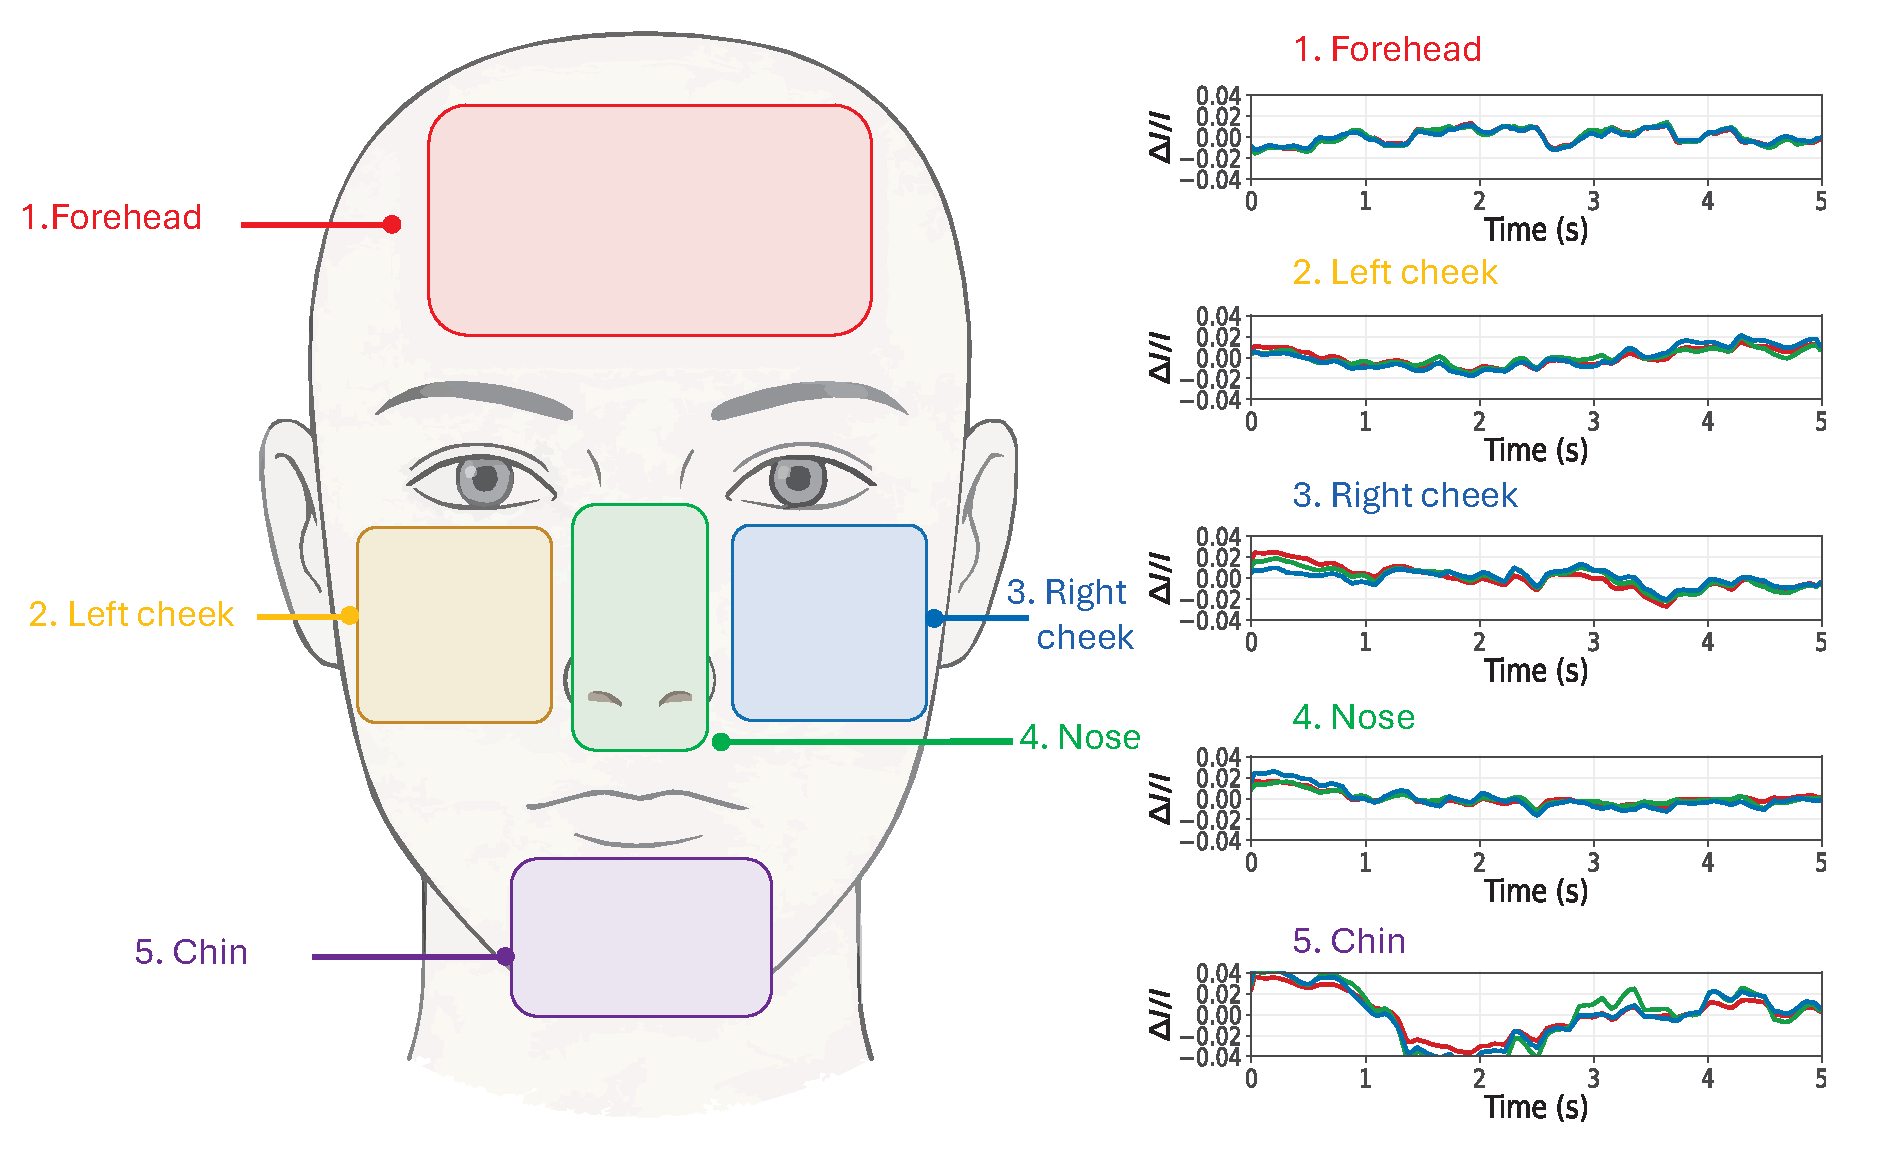
\includegraphics[width=0.98\textwidth]{f2.eps}
\caption{Architecture of RT-MRCPNet. A facial clip is converted into multi-region RGB sequences, encoded by a shared temporal encoder, adaptively aggregated by temporal and region attention, and classified as stress or non-stress.}
\label{fig:overview}
\end{figure}

\subsection{Training Objective}

We train the model with cross-entropy loss. Let $p_c=\mathrm{softmax}(o)_c$ be the predicted probability of class $c$. The loss is
\begin{equation}
    \mathcal{L}_{cls} = -\sum_{c=1}^{2} y_c \log p_c
\end{equation}
where $y_c$ is the one-hot ground-truth label for class $c$. We use only classification supervision, so the comparison focuses on regional RGB dynamics and attention aggregation rather than auxiliary reconstruction or contrastive objectives.

\section{Experiments}

\subsection{Dataset and Label Definition}

The main experiments target social-stress facial video data. For UBFC-Phys-style data, each subject includes rest, speech, and arithmetic tasks. Following common social-stress protocol interpretation, rest is treated as non-stress, while speech and arithmetic are treated as stress:
\begin{equation}
    \mathrm{T1}=0,\quad \mathrm{T2/T3}=1
\end{equation}
This binary setting is clear and reproducible, and matches the focus of whether video alone can distinguish resting clips from social-stress tasks.


\subsection{Subject-Independent Protocol}

All experiments use a subject-independent split, so clips from the same subject cannot appear in both training and test sets. Otherwise, the model may learn identity appearance rather than stress-related dynamics. The fixed split uses 70\% of subjects for training, 15\% for validation, and 15\% for testing. Validation is used only for model selection, and the test set only for final reporting. Subject IDs or random seeds are recorded for reproducibility.

\subsection{Implementation Details}

Faces are cropped and resized to $128 \times 128$. Each video is divided into fixed-length clips with $T=160$ by default. We use five fixed facial regions and extract a temporally normalized per-frame RGB mean sequence from each region. The hidden dimension is 128. The optimizer is AdamW, the initial learning rate is $10^{-3}$, the batch size is 64, and the main experiments train for 30 epochs. The best checkpoint is selected by validation F1-score. Experiments are conducted on a single RTX 5090 GPU with PyTorch.

\subsection{Evaluation Metrics}

We report Accuracy, F1-score, and AUC, and use a confusion matrix to show the final error distribution. Since stress recognition may involve class imbalance, F1-score and AUC are more informative than Accuracy alone. The stress state is treated as the positive class.

\subsection{Comparison Experiments}

The comparison experiments follow a unified protocol. Whenever possible, all methods use the same input source, subject-independent split, clip construction, and evaluation code. These comparisons test whether multi-region temporal representation with attention fusion improves performance when all inputs are restricted to facial RGB video. The baselines range from simple color-sequence models to video temporal and rPPG-related models.

\begin{itemize}
    \item Full-face RGB temporal network: the five regional sequences are averaged into a whole-face RGB sequence and then temporally encoded.
    \item Single-region RGB temporal networks: forehead, left cheek, right cheek, nose, and chin sequences are used separately to observe differences among facial regions.
    \item Fixed multi-region fusion: multiple regional RGB sequences are retained, but they are fused by non-adaptive concatenation or averaging, without attention.
    \item Traditional rPPG feature classifiers: POS~\cite{wang2017pos} or CHROM~\cite{dehaan2013chrom} extracts facial color signals, from which heart-rate and HRV features are classified by a support vector machine or random forest.
    \item Lightweight video temporal baselines: a compact CNN-LSTM~\cite{ziaratnia2024cctlstm} or 3D CNN~\cite{tran2015c3d} takes cropped facial clips as input and outputs the stress class.
    \item Existing rPPG backbone with a stress head: the output head of PhysNet~\cite{yu2019physnet}, a representative rPPG model, is replaced with a stress classification head.
    \item RT-MRCPNet: the proposed method, using multi-region RGB sequences with temporal attention and region attention for adaptive fusion.
\end{itemize}

\begin{table}[!htbp]
\caption{Comparison experiments under the UBFC-Phys subject-independent protocol. All models use facial RGB video and share the same clip length, split, and evaluation code. ACC, F1, and AUC are reported in percentages (\%).}
\label{tab:main_results}
\centering
\small
\begin{tabular}{p{3.9cm}p{4.45cm}ccc}
\toprule
Method & Input & ACC & F1 & AUC \\
\midrule
Full-face RGB temporal network & Whole-face averaged RGB sequence & 82.24 & 87.56 & 87.20 \\
\addlinespace[0.1em]
Forehead single-region temporal network & Forehead RGB sequence & 75.21 & 82.06 & 79.36 \\
Left-cheek single-region temporal network & Left-cheek RGB sequence & 73.88 & 80.76 & 77.15 \\
Right-cheek single-region temporal network & Right-cheek RGB sequence & 64.20 & 76.09 & 59.82 \\
Nose single-region temporal network & Nose RGB sequence & 78.35 & 83.74 & 85.96 \\
Chin single-region temporal network & Chin RGB sequence & 80.72 & 86.05 & 85.40 \\
\addlinespace[0.1em]
Fixed multi-region fusion & Five ROI RGB sequences, fixed fusion & 80.72 & 85.67 & 89.12 \\
\addlinespace[0.1em]
rPPG features + support vector machine & Heart-rate/HRV hand-crafted features & 77.87 & 84.18 & 76.79 \\
rPPG features + random forest & Heart-rate/HRV hand-crafted features & 77.02 & 84.43 & 75.60 \\
\addlinespace[0.1em]
Lightweight CNN-LSTM & ROI RGB temporal tensor & 67.33 & 76.82 & 62.73 \\
Lightweight 3D CNN & ROI RGB temporal tensor & 70.75 & 80.60 & 70.70 \\
\addlinespace[0.1em]
PhysNet + stress classification head & Full-face RGB/rPPG-related features & 80.63 & 86.61 & 87.64 \\
\addlinespace[0.1em]
RT-MRCPNet & Five ROI RGB sequences, attention fusion & \textbf{86.42} & \textbf{90.27} & \textbf{93.07} \\
\bottomrule
\end{tabular}
\end{table}


Table~\ref{tab:main_results} shows that RT-MRCPNet obtains the highest ACC, F1-score, and AUC among all baselines. Compared with the full-face RGB temporal network, it improves the three metrics by 4.18, 2.71, and 5.87 percentage points; compared with fixed multi-region fusion, the gains are 5.70, 4.60, and 3.95 points. The improvement therefore comes not only from using multiple ROIs, but also from selecting reliable time positions and discriminative facial regions. The single-region results show clear regional differences: chin and nose outperform cheek-only sequences in this split, but no single region reaches adaptive multi-region performance.

Fig.~\ref{fig:region_signal_diversity} shows color-pulse differences among the five facial ROIs. The regions differ in amplitude, stability, and disturbance level, consistent with the single-region results in Table~\ref{tab:main_results}. This indicates that whole-face averaging or fixed fusion can lose useful local evidence.

\begin{figure}[!htbp]
\centering
\IfFileExists{f3.eps}{%
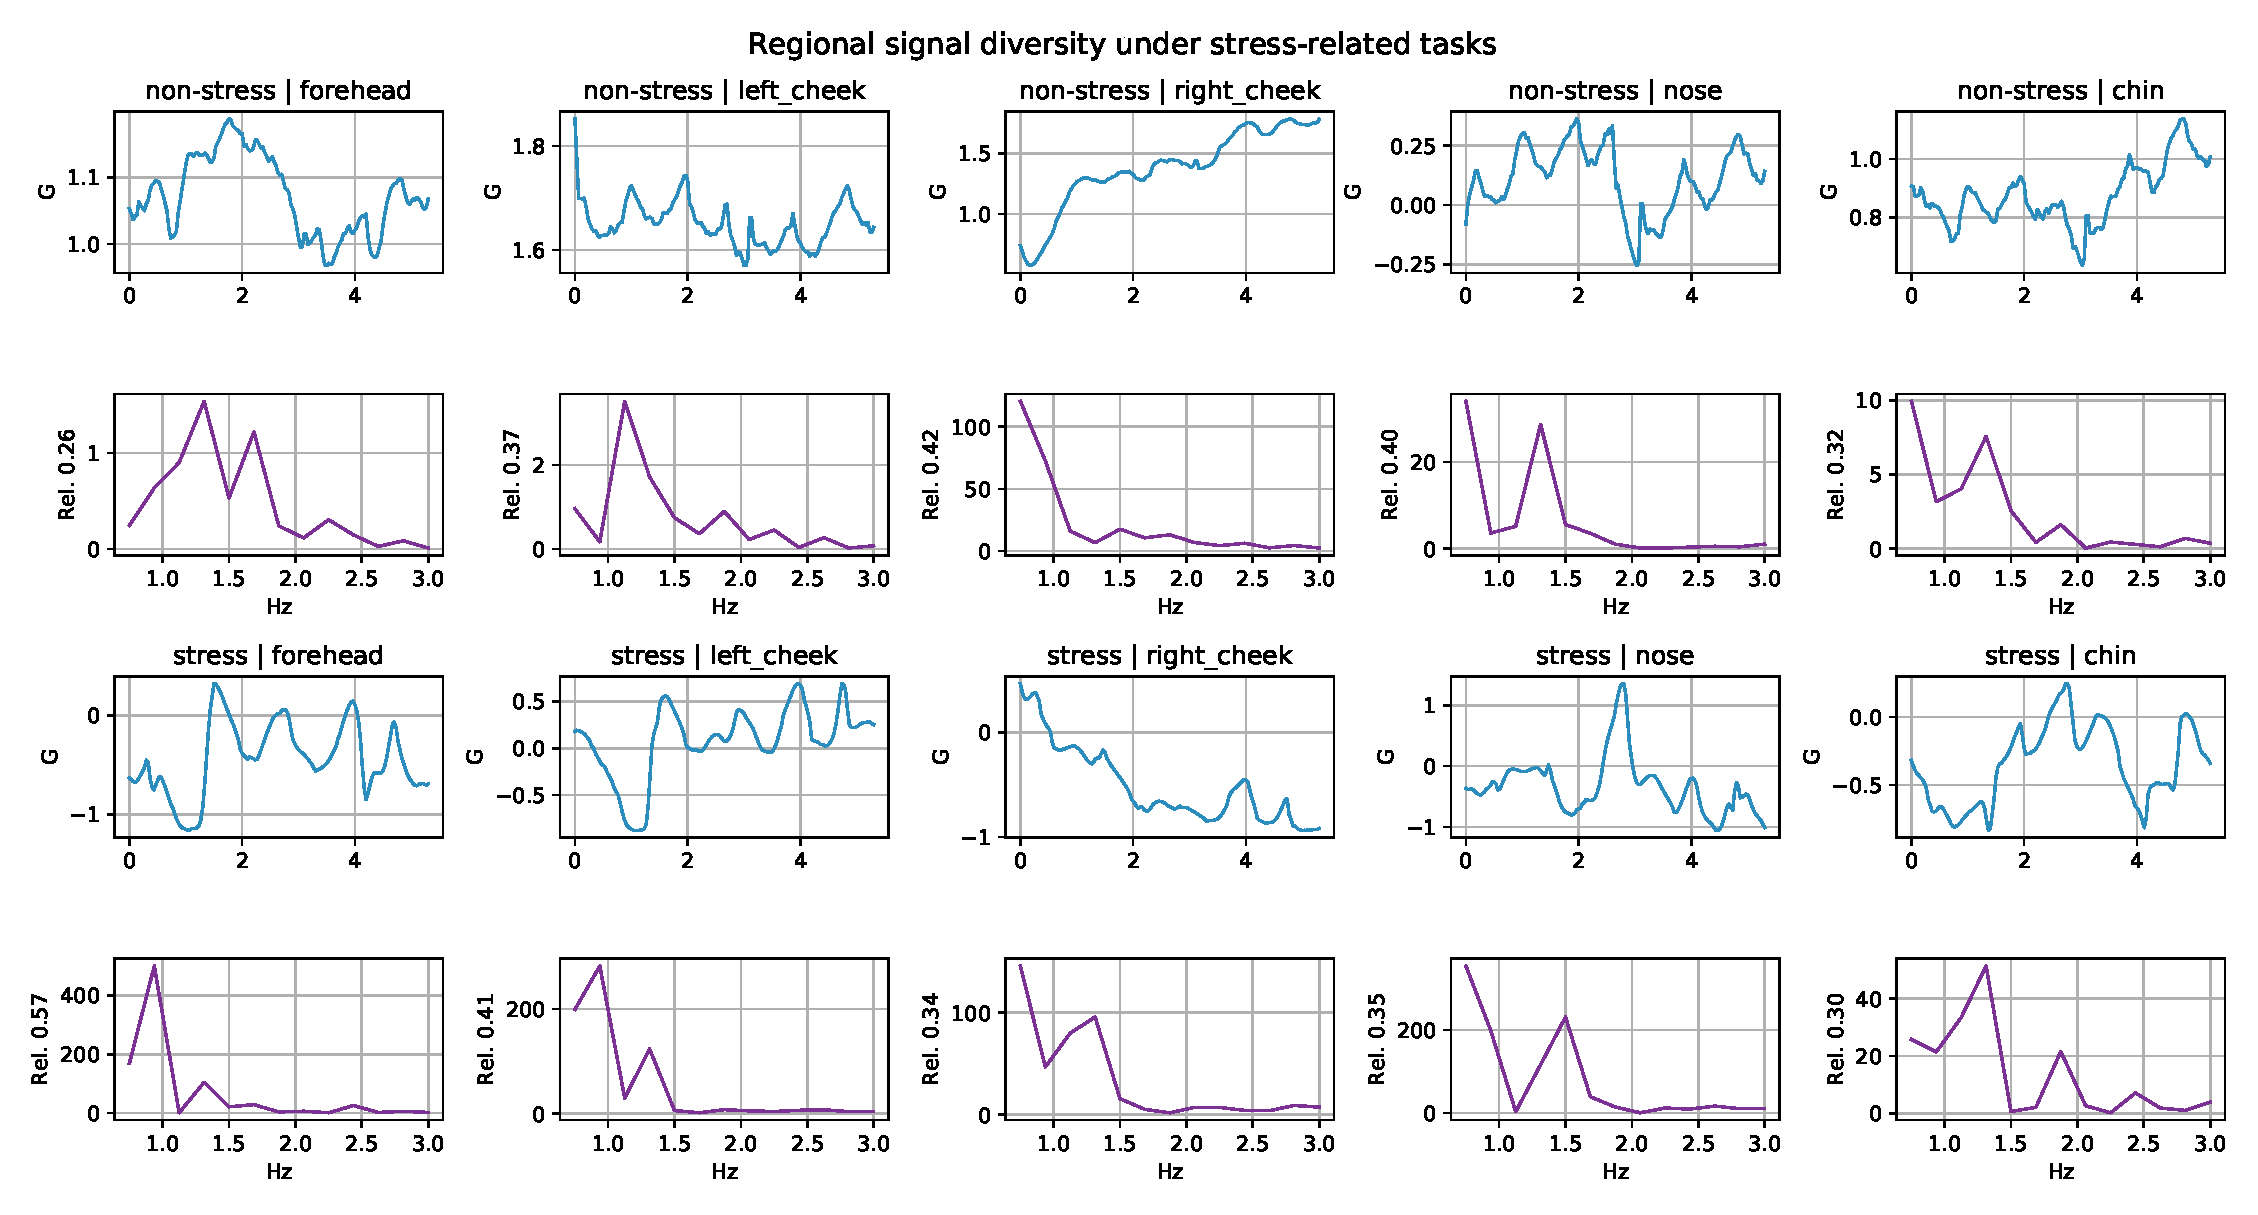
\includegraphics[width=\textwidth,height=0.32\textheight,keepaspectratio]{f3.eps}%
}{%
\figplaceholder{Figure 3 Region Signal Diversity Visualization}{Color pulse signal differences across five facial ROIs.}%
}
\caption{Region signal diversity visualization. Different facial regions show different signal amplitude, shape, and stability, indicating regionally uneven stress-related cues.}
\label{fig:region_signal_diversity}
\end{figure}

Fig.~\ref{fig:attention_reliability} illustrates the relationship between attention weights and input reliability. Temporal attention distinguishes stable and disturbed time positions, while region attention reflects each facial area's contribution to the final decision, explaining the advantage over fixed fusion.

\begin{figure}[!htbp]
\centering
\IfFileExists{f4.eps}{%
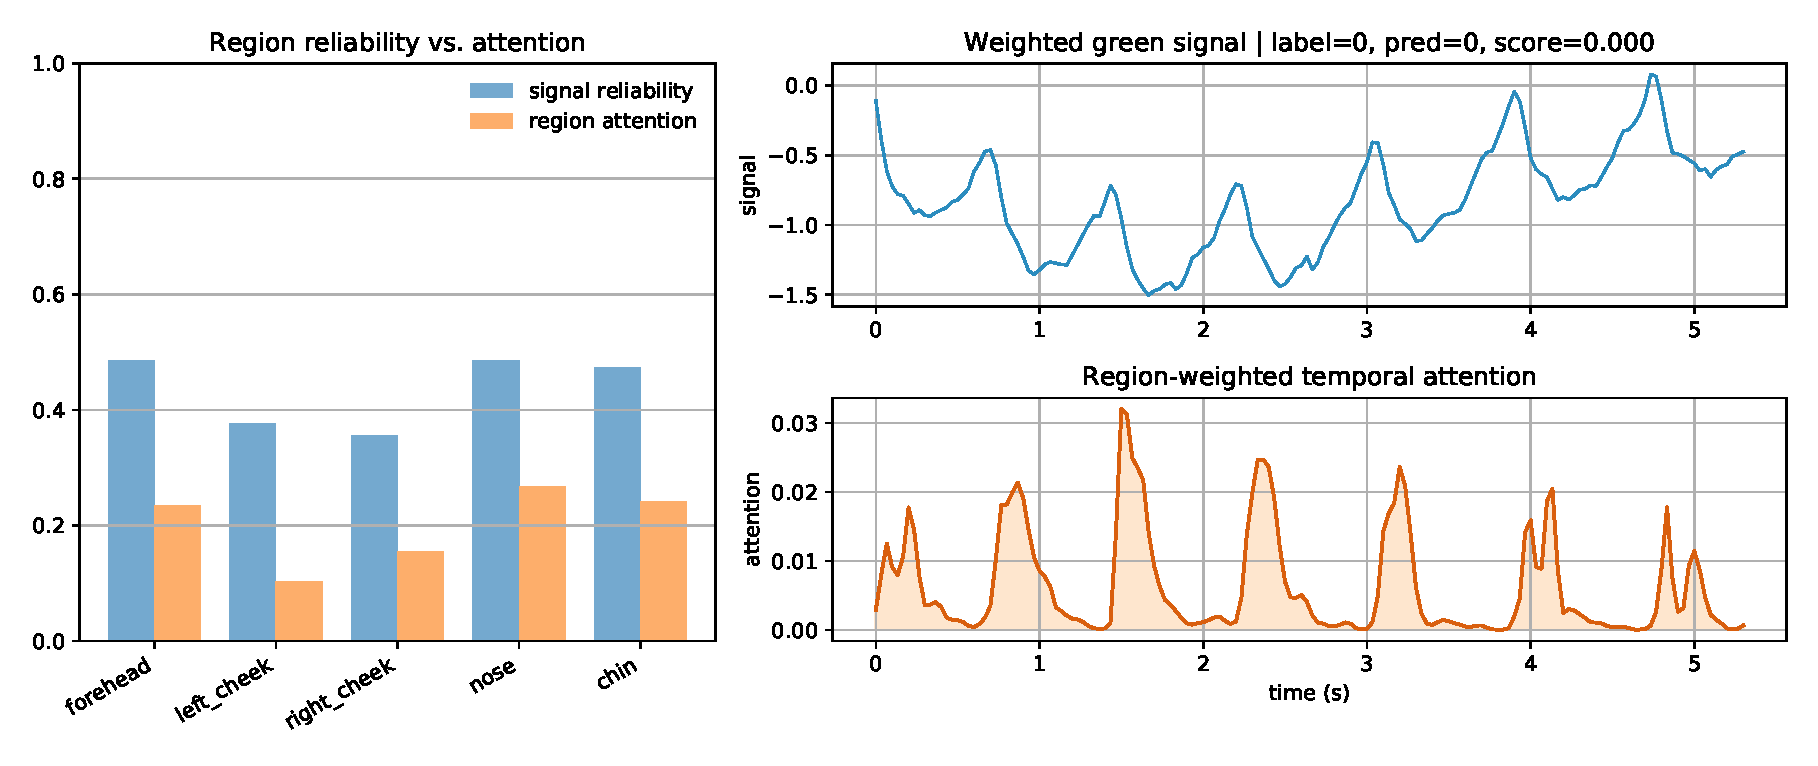
\includegraphics[width=\textwidth,height=0.32\textheight,keepaspectratio]{f4.eps}%
}{%
\figplaceholder{Figure 4 Attention Reliability Visualization}{Temporal attention changes and region attention weights in representative clips.}%
}
\caption{Attention reliability visualization. Temporal and region attention distributions show how RT-MRCPNet reduces unstable segments or low-quality regions and highlights reliable discriminative cues.}
\label{fig:attention_reliability}
\end{figure}

\subsection{Ablation Study}

The ablation study uses the same protocol as Table~\ref{tab:main_results}. Unlike the comparison experiments, it removes specific attention modules from RT-MRCPNet to examine each component's contribution.

Table~\ref{tab:ablation} shows that temporal attention is the stronger individual contributor in this split. Removing both attention modules reduces the model to fixed multi-region fusion. Adding temporal attention brings clear gains in ACC, F1-score, and AUC, while region attention alone gives only small ACC and F1-score improvements. Combining both attention stages yields the highest ACC and F1-score, with AUC close to the temporal-only version. Thus, temporal reliability modeling provides the main robustness gain, and region attention further improves discriminative ability.

\begin{table}[!htbp]
\caption{Ablation study of RT-MRCPNet. ACC, F1, and AUC are reported in percentages (\%).}
\label{tab:ablation}
\centering
\begin{tabular}{lccc}
\toprule
Model variant & ACC & F1 & AUC \\
\midrule
Without attention & 80.72 & 85.67 & 89.12 \\
Temporal attention only & 85.57 & 89.78 & \textbf{93.16} \\
Region attention only & 81.10 & 85.69 & 88.84 \\
Full RT-MRCPNet & \textbf{86.42} & \textbf{90.27} & 93.07 \\
\bottomrule
\end{tabular}
\end{table}

\subsection{Complexity Analysis}

RT-MRCPNet uses compact regional RGB sequences rather than full facial video frames. For a clip of length $T$, resolution $H \times W$, and $C$ color channels, the input size of a full-frame model is $\mathcal{O}(T H W C)$. After regional color pooling, RT-MRCPNet keeps only the mean color sequences of $K$ regions, reducing the input size to $\mathcal{O}(K T C)$. Since $K \ll H W$, the representation significantly reduces spatial redundancy before entering the neural network.

Let $D$ be the hidden dimension, $q$ the one-dimensional convolution kernel size, $L$ the number of encoder layers, and $B$ the batch size. The shared temporal encoder processes $B K$ regional sequences with main complexity $\mathcal{O}(B K L T q D^2)$, while temporal and region attention add $\mathcal{O}(B K T D + B K D)$. Thus, computation grows with the number of regions $K$ and clip length $T$, not directly with image area $H W$.

Table~\ref{tab:complexity} reports the parameter count and average forward inference time of representative methods. RT-MRCPNet has a parameter count comparable to the full-face RGB temporal network and clearly lower than CNN-LSTM, while remaining lightweight. Its inference time is higher than full-face RGB and the PhysNet/EfficientPhys classification head because it processes five ROIs separately and computes temporal and region attention. Nevertheless, the cost remains below $0.1$ ms, much smaller than typical video preprocessing and face detection overhead. Compared with the lightweight 3D CNN, RT-MRCPNet avoids directly modeling full spatial frames at a similar inference time and concentrates computation on regional color dynamics and adaptive fusion, giving a better trade-off between complexity and recognition performance.

\begin{table}
\caption{Model complexity comparison. Inference time denotes the average forward time per clip.}
\label{tab:complexity}
\centering
\begin{tabular}{lcc}
\toprule
Method & Parameters & Inference time \\
\midrule
Full-face RGB temporal network & 0.069M & 0.0243 ms \\
Lightweight CNN-LSTM & 0.146M & 0.0439 ms \\
Lightweight 3D CNN & 0.019M & 0.0832 ms \\
PhysNet/EfficientPhys + stress head & 0.073M & 0.0215 ms \\
RT-MRCPNet & 0.069M & 0.0817 ms \\
\bottomrule
\end{tabular}
\end{table}

\section{Conclusion}

This paper presents RT-MRCPNet, a lightweight region-temporal attention network for contactless stress recognition. It converts facial video into multi-region RGB temporal sequences, models local color dynamics with a shared encoder, and aggregates information through temporal and region attention. Under a subject-independent protocol, RT-MRCPNet achieves 86.42\% ACC, 90.27\% F1-score, and 93.07\% AUC. The ablation and complexity results show that the two attention stages provide complementary gains with low computational cost. Future work will explore adaptive ROI definitions, finer-grained stress labels, and multimodal fusion.

\begingroup
\bibliographystyle{splncs04}
\bibliography{references}
\endgroup

\end{document}
